\chapter{Векторы, матрицы и линейные системы}\markright{Глава 18}
\section*{Координаты точки и координаты перемещения}
\par\addvspace{5pt}\begin{lrbox}{\CatFlowBox}\begin{minipage}[t]{\linewidth}
\setlength{\parskip}{5pt}\setlength{\columnsep}{4.5mm}\setlength{\intextsep}{0pt}
\begin{wrapfigure}[13]{r}{54mm}
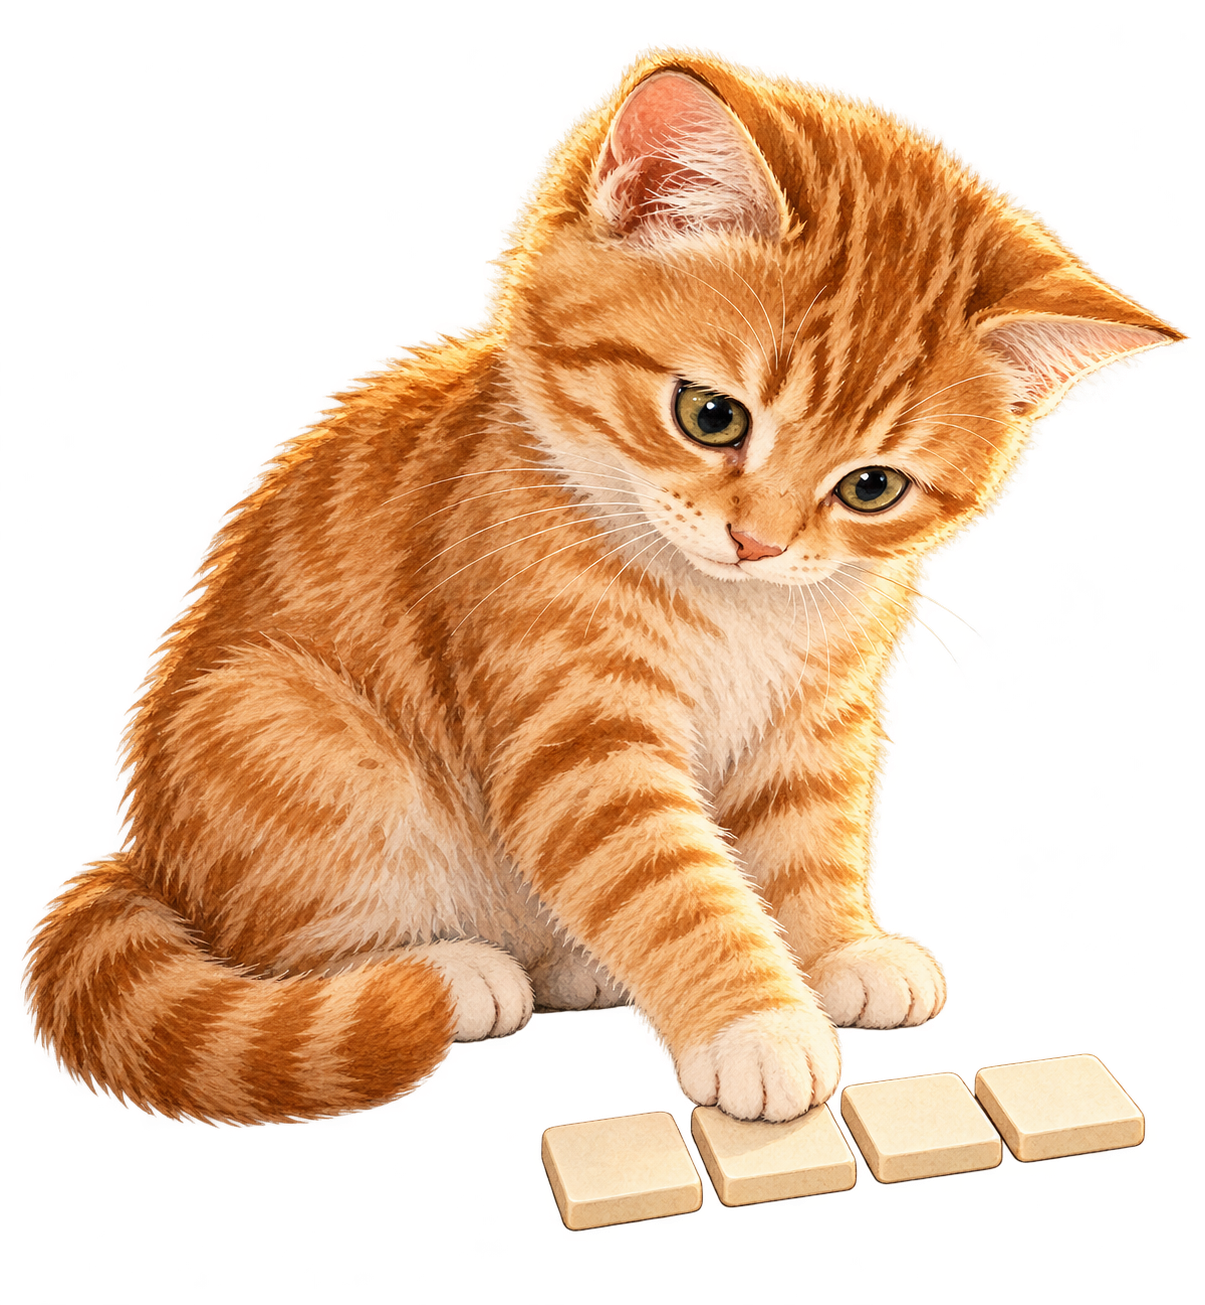
\includegraphics[width=54mm,height=58mm,keepaspectratio]{images/unique/art-01.png}
\end{wrapfigure}
Пара чисел может описывать точку плоскости, а может описывать перемещение. Точка отвечает на вопрос «где?», вектор — на вопрос «на сколько и в каком направлении?». Все координаты и коэффициенты в этой главе действительные. Основные модели — \(\mathbb R^2\) и \(\mathbb R^3\); абстрактные векторные пространства пока не понадобятся.
\par\WFclear\end{minipage}\end{lrbox}%
\ifdim\dimexpr\ht\CatFlowBox+\dp\CatFlowBox\relax<64mm\dp\CatFlowBox=\dimexpr64mm-\ht\CatFlowBox\relax\fi%
\noindent\usebox{\CatFlowBox}\par\addvspace{5pt}
\begin{definition}
\term{Координатный вектор} (coordinate vector) плоскости — упорядоченная пара \(\mathbf u=(u_1;u_2)\in\mathbb R^2\). В пространстве это тройка \(\mathbf u=(u_1;u_2;u_3)\in\mathbb R^3\). Два вектора равны, если совпадают все соответствующие координаты.
\end{definition}
Вектор перемещения из \(A=(a_1;a_2)\) в \(B=(b_1;b_2)\) имеет координаты \(\overrightarrow{AB}=(b_1-a_1;b_2-a_2)\). Например, из \((2;-1)\) в \((-1;3)\) нужно сместиться на \((-3;4)\). Одинаковые перемещения можно начинать в разных точках; их координаты от этого не меняются.

\begin{definition}
\term{Сумма векторов} (vector sum) и \term{умножение вектора на число} (scalar multiplication) выполняются по координатам:
\[
\begin{aligned}
(u_1;u_2)+(v_1;v_2)&=(u_1+v_1;u_2+v_2),\\
\lambda(u_1;u_2)&=(\lambda u_1;\lambda u_2).
\end{aligned}
\]
В \(\mathbb R^3\) то же правило применяется и к третьей координате. \term{Нулевой вектор} (zero vector) \(\mathbf0\) имеет все координаты нулевыми. \term{Противоположный вектор} (additive inverse) равен \(-\mathbf u\).
\end{definition}
Сумма описывает два последовательных перемещения. По правилу треугольника начало второго перемещения помещают в конец первого. Например, \((3;0)+(0;4)=(3;4)\). Умножение на положительное число растягивает или сжимает перемещение, отрицательный множитель дополнительно меняет направление; множитель \(0\) даёт нулевой вектор. Переместительное и сочетательное свойства сложения, а также распределительные свойства следуют из соответствующих равенств для каждой координаты.

\begin{definition}
\term{Длина вектора, или евклидова норма} (Euclidean norm) определяется формулами
\[
\|\mathbf u\|=\sqrt{u_1^2+u_2^2}\quad\text{в }\mathbb R^2,
\qquad
\|\mathbf u\|=\sqrt{u_1^2+u_2^2+u_3^2}\quad\text{в }\mathbb R^3.
\]
\term{Скалярное произведение} (dot product) векторов одинаковой размерности равно сумме произведений соответствующих координат. Например, в \(\mathbb R^2\) это \(\mathbf u\cdot\mathbf v=u_1v_1+u_2v_2\). Векторы называют \term{ортогональными} (orthogonal), если их скалярное произведение равно нулю.
\end{definition}
Формулы длины следуют из теоремы Пифагора; для трёх координат её применяют сначала в горизонтальной плоскости, затем с учётом высоты. Расстояние между точками равно длине вектора их разности. Векторы \((3;4)\) и \((4;-3)\) ортогональны, поскольку \(3\cdot4+4\cdot(-3)=0\). Неравенство Коши--Буняковского из предыдущей главы теперь читается как \(|\mathbf u\cdot\mathbf v|\le\|\mathbf u\|\|\mathbf v\|\) для векторов плоскости.

\section*{Линейная комбинация и зависимость}
\begin{definition}
\term{Линейная комбинация} (linear combination) векторов \(\mathbf v_1,\ldots,\mathbf v_k\) одинаковой размерности — вектор вида \(\lambda_1\mathbf v_1+\cdots+\lambda_k\mathbf v_k\), где коэффициенты \(\lambda_i\) действительные.
\end{definition}
\begin{definition}
Векторы \(\mathbf v_1,\ldots,\mathbf v_k\) \term{линейно зависимы} (linearly dependent), если существуют коэффициенты, не все равные нулю, для которых
\[
\lambda_1\mathbf v_1+\cdots+\lambda_k\mathbf v_k=\mathbf0.
\]
Они \term{линейно независимы} (linearly independent), если нулевая комбинация получается только при \(\lambda_1=\cdots=\lambda_k=0\).
\end{definition}
Два ненулевых вектора зависимы ровно тогда, когда один является числовым множителем другого. Действительно, из \(\alpha\mathbf u+\beta\mathbf v=\mathbf0\) при \(\beta\ne0\) получаем \(\mathbf v=-\frac\alpha\beta\mathbf u\); если \(\beta=0\), то для нетривиальной зависимости \(\alpha\ne0\), что дало бы запрещённое \(\mathbf u=\mathbf0\). Обратно, равенство \(\mathbf v=t\mathbf u\) даёт нетривиальную комбинацию \(t\mathbf u-\mathbf v=\mathbf0\). Наличие нулевого вектора всегда делает набор зависимым: достаточно поставить при нём коэффициент \(1\), а при остальных \(0\).

\begin{definition}
\term{Базис} (basis) в \(\mathbb R^2\) или \(\mathbb R^3\) — упорядоченный набор векторов, через который любой вектор соответствующей модели представляется единственной линейной комбинацией. \term{Стандартный базис} (standard basis) плоскости состоит из \(\mathbf e_1=(1;0)\), \(\mathbf e_2=(0;1)\); в пространстве добавляют третью координату и \(\mathbf e_3=(0;0;1)\).
\end{definition}
Например, \((x;y)=x\mathbf e_1+y\mathbf e_2\), и коэффициенты единственны, потому что равенство векторов означает равенство каждой координаты. В \(\mathbb R^3\) аналогично \((x;y;z)=x\mathbf e_1+y\mathbf e_2+z\mathbf e_3\). Базис позволяет задавать вектор списком коэффициентов. В другом базисе этот список может измениться, хотя само геометрическое перемещение останется прежним.

\section*{Матрица: несколько линейных формул в одной записи}
\begin{definition}
\term{Матрица} (matrix) размера \(m\times n\) — прямоугольная таблица чисел с \(m\) строками и \(n\) столбцами. Элемент \(a_{ij}\) расположен в строке \(i\), столбце \(j\). Матрица \term{квадратная} (square), если \(m=n\).
\end{definition}
Матрицы одинакового размера складывают поэлементно и умножают на число поэлементно. Для матриц разных размеров сумма не определена. Например,
\[
\begin{pmatrix}1&2\\0&-1\end{pmatrix}
+2\begin{pmatrix}3&0\\1&2\end{pmatrix}
=\begin{pmatrix}7&2\\2&3\end{pmatrix}.
\]
\begin{definition}
\term{Произведение матрицы на вектор} (matrix--vector product) получают, умножая каждую строку на столбец координат:
\[
\begin{pmatrix}a&b\\c&d\end{pmatrix}
\begin{pmatrix}x\\y\end{pmatrix}
=\begin{pmatrix}ax+by\\cx+dy\end{pmatrix}.
\]
Для матрицы \(m\times n\) входной столбец должен содержать \(n\) координат, выходной содержит \(m\).
\end{definition}
Если \(A\) имеет столбцы \(\mathbf a_1,\ldots,\mathbf a_n\), то \(A\mathbf x=x_1\mathbf a_1+\cdots+x_n\mathbf a_n\): это одна и та же формула, прочитанная по столбцам вместо строк. Поэтому задача \(A\mathbf x=\mathbf b\) спрашивает, можно ли получить \(\mathbf b\) как комбинацию столбцов \(A\) и единственны ли коэффициенты.

\par\addvspace{5pt}\begin{lrbox}{\CatFlowBox}\begin{minipage}[t]{\linewidth}
\setlength{\parskip}{5pt}\setlength{\columnsep}{4.5mm}\setlength{\intextsep}{0pt}
\begin{wrapfigure}[11]{r}{54mm}
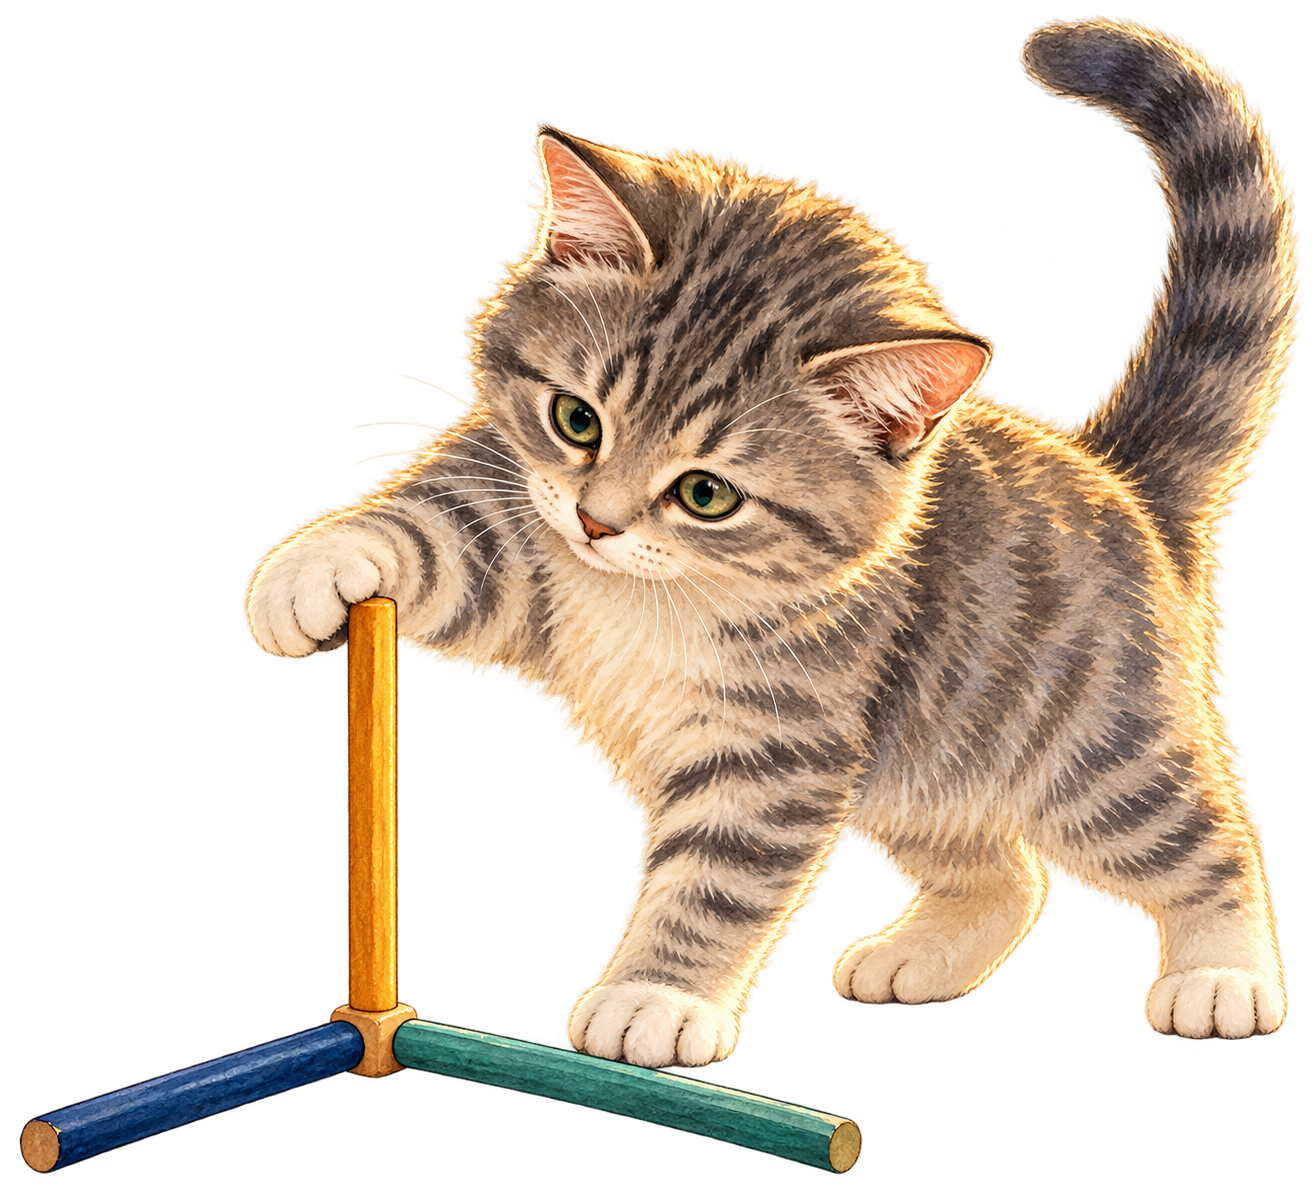
\includegraphics[width=54mm,height=58mm,keepaspectratio]{images/unique/art-47.png}
\end{wrapfigure}
Матричная запись помогает одновременно видеть несколько связей между величинами. Строка описывает, как вычисляется один результат, а столбец показывает вклад одной входной величины во все результаты. Например, в таблице расхода продуктов столбцы могут соответствовать двум видам наборов, а строки — разным ингредиентам. Умножение на столбец количеств наборов сразу даёт общий расход каждого ингредиента. В геометрии те же числа описывают изменение координат: один столбец задаёт образ первого стандартного базисного вектора, другой — второго. Поэтому смысл произведения полезно проверять до вычислений: сколько величин подаётся на вход, сколько должно получиться на выходе и в каких единицах они измеряются. Такая проверка часто обнаруживает перепутанный порядок матриц или строк раньше, чем появляется ошибочный численный ответ.
\par\WFclear\end{minipage}\end{lrbox}%
\ifdim\dimexpr\ht\CatFlowBox+\dp\CatFlowBox\relax<64mm\dp\CatFlowBox=\dimexpr64mm-\ht\CatFlowBox\relax\fi%
\noindent\usebox{\CatFlowBox}\par\addvspace{5pt}
\begin{definition}
\term{Произведение матриц} (matrix product) \(C=AB\) определено, если число столбцов \(A\) равно числу строк \(B\). При размерах \(m\times n\) и \(n\times p\) результат имеет размер \(m\times p\), причём
\[
c_{ij}=\sum_{k=1}^{n}a_{ik}b_{kj}.
\]
То есть берут скалярное произведение строки первой матрицы и столбца второй.
\end{definition}
Например, для
\[
A=\begin{pmatrix}1&1\\0&1\end{pmatrix},\qquad
B=\begin{pmatrix}1&0\\1&1\end{pmatrix}
\]
получаем
\[
AB=\begin{pmatrix}2&1\\1&1\end{pmatrix},\qquad
BA=\begin{pmatrix}1&1\\1&2\end{pmatrix}.
\]
Значит, умножение матриц в общем случае некоммутативно. Иногда одно из произведений \(AB\), \(BA\) даже не определено из-за размеров.

\section*{Матрица как линейное отображение}
\begin{definition}
\term{Линейное отображение} (linear map) в координатных моделях — отображение \(T\), сохраняющее линейные комбинации двух векторов:
\[
T(\alpha\mathbf u+\beta\mathbf v)
=\alpha T(\mathbf u)+\beta T(\mathbf v)
\]
для любых допустимых векторов и действительных \(\alpha,\beta\).
\end{definition}
При \(\alpha=\beta=0\) определение даёт \(T(\mathbf0)=\mathbf0\). Поэтому несохранение нулевого вектора сразу опровергает линейность.
\begin{theorem}[Линейность матричного действия и композиция]
Отображение \(T_A(\mathbf x)=A\mathbf x\) линейно. Для согласованных размеров последовательное применение \(T_B\), затем \(T_A\) задаётся матрицей \(AB\):
\[
A(B\mathbf x)=(AB)\mathbf x.
\]
\end{theorem}
\begin{proof}
В каждой строке распределительный закон даёт
\(\sum_j a_{ij}(\alpha u_j+\beta v_j)=\alpha\sum_j a_{ij}u_j+\beta\sum_j a_{ij}v_j\), что доказывает линейность. Для композиции \(i\)-я координата левой части равна
\[
\sum_k a_{ik}\left(\sum_j b_{kj}x_j\right)
=\sum_j\left(\sum_k a_{ik}b_{kj}\right)x_j.
\]
Все суммы конечные; перестановка слагаемых и раскрытие скобок допустимы. Внутренняя сумма — элемент \((AB)_{ij}\), поэтому получена \(i\)-я координата правой части.
\end{proof}
Так, \(A=\begin{pmatrix}2&1\\0&1\end{pmatrix}\) действует по правилу \(T_A(x;y)=(2x+y;y)\). Вершины единичного квадрата \((0;0),(1;0),(1;1),(0;1)\) переходят в \((0;0),(2;0),(3;1),(1;1)\). Матрица \(R=\begin{pmatrix}0&-1\\1&0\end{pmatrix}\) задаёт поворот плоскости на \(90^\circ\) против часовой стрелки: \((x;y)\mapsto(-y;x)\). На единичной окружности это следует из формул для \(\cos(\alpha+\frac\pi2)\) и \(\sin(\alpha+\frac\pi2)\), а умножение на радиус даёт то же для любой точки. Напротив, перенос \((x;y)\mapsto(x+1;y)\) нелинеен: он не сохраняет нулевой вектор.

\section*{Метод Гаусса и смысл преобразования строк}
\begin{definition}
\term{Линейная система} (linear system) — система уравнений первой степени по неизвестным с постоянными коэффициентами; её матричная запись — \(A\mathbf x=\mathbf b\). \term{Расширенная матрица} (augmented matrix) \((A\mid\mathbf b)\) содержит также столбец правых частей.
\end{definition}
Например, \(x+y=3\), \(x-y=1\) записываются как \(\begin{pmatrix}1&1&\mid&3\\1&-1&\mid&1\end{pmatrix}\). Вертикальная черта отделяет правые части и не является коэффициентом.

\begin{theorem}[Равносильные преобразования строк]
Множество решений системы сохраняется при перестановке двух уравнений, умножении уравнения на ненулевое число и прибавлении к одному уравнению другого, умноженного на любое число. При преобразовании строки меняют также её правую часть.
\end{theorem}
\begin{proof}
Перестановка меняет только порядок условий и обращается той же перестановкой. Умножение на \(\lambda\ne0\) обращается умножением на \(\frac1\lambda\), поэтому обе записи требуют одного и того же. Если к уравнению \(i\) прибавили \(\lambda\) раз уравнение \(j\), всякое старое решение удовлетворяет новому уравнению. Обратно, уравнение \(j\) осталось неизменным: вычитая его с множителем \(\lambda\), восстанавливаем старое уравнение \(i\). Значит, каждое новое решение является старым.
\end{proof}
\begin{definition}
\term{Ступенчатый вид} (row echelon form) матрицы означает: нулевые строки стоят ниже ненулевых, а первый ненулевой элемент каждой следующей ненулевой строки расположен правее такого элемента предыдущей. Эти первые элементы называют \term{ведущими элементами} (pivots), их позиции — ведущими позициями.
\end{definition}
\term{Метод Гаусса} (Gaussian elimination) последовательно выбирает ненулевой ведущий коэффициент, при необходимости переставляет строки и вычитанием кратных обнуляет элементы под ним. Далее тот же процесс продолжают в меньшем прямоугольнике справа и снизу. Число строк и столбцов конечно, поэтому получится ступенчатая форма. Затем неизвестные находят в обратном порядке — от нижнего ненулевого уравнения к верхнему.

Например, система
\[
\begin{cases}
x+y+z=6,\\
2x+y+z=7,\\
x+2y+3z=14
\end{cases}
\]
после вычитания удвоенного первого уравнения из второго и первого из третьего превращается в
\[
\begin{cases}
x+y+z=6,\\
-y-z=-5,\\
y+2z=8.
\end{cases}
\]
Сложив два последних уравнения, получаем \(z=3\). Затем \(y=2\) и \(x=1\). Проверка во всех исходных уравнениях даёт \(6\), \(7\), \(14\), как требуется.

\begin{definition}
Система \term{совместна} (consistent), если имеет хотя бы одно решение, и \term{несовместна} (inconsistent), если решений нет. В ступенчатой форме \term{ведущие переменные} (pivot variables) соответствуют ведущим позициям матрицы коэффициентов; остальные \term{свободные переменные} (free variables) можно выбирать как параметры, если система совместна. \term{Ранг матрицы} (matrix rank), обозначаемый \(\operatorname{rank}A\), — наибольшее число её линейно независимых столбцов. Для нулевой матрицы ранг равен \(0\). Ниже доказано, как прочитать это число по ступенчатой форме.
\end{definition}
\begin{theorem}[Чтение решений из ступенчатой формы]
Если преобразованная система содержит строку \(0=\gamma\) с \(\gamma\ne0\), она несовместна. Если таких строк нет, система совместна: свободным переменным можно независимо присвоить любые действительные значения, после чего ведущие переменные единственным образом находятся обратной подстановкой. В частности, при отсутствии свободных переменных решение единственно.
\end{theorem}
\par\addvspace{5pt}\begin{lrbox}{\CatFlowBox}\begin{minipage}[t]{\linewidth}
\setlength{\parskip}{5pt}\setlength{\columnsep}{4.5mm}\setlength{\intextsep}{0pt}
\begin{wrapfigure}[11]{l}{54mm}
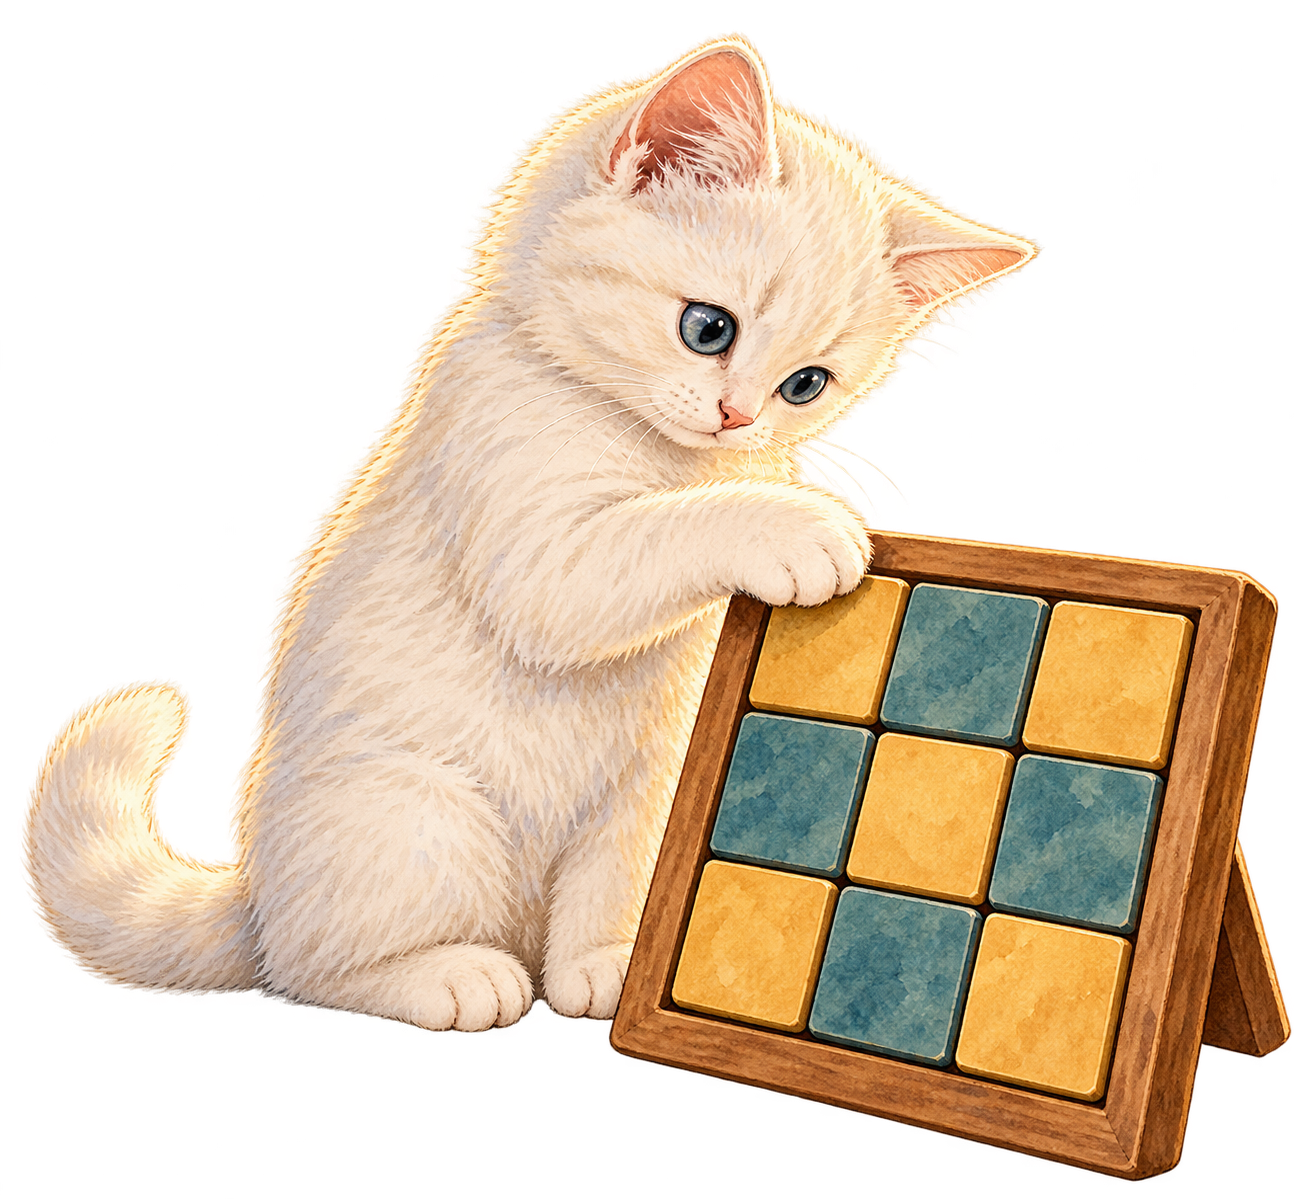
\includegraphics[width=54mm,height=58mm,keepaspectratio]{images/unique/art-48.png}
\end{wrapfigure}
\textit{Доказательство.} Строку \(0=\gamma\ne0\) не удовлетворяет ни один набор неизвестных. Если её нет, нулевые строки дают только \(0=0\) и не накладывают условий. В последнем ненулевом уравнении все переменные правее ведущей свободны; после их выбора деление на ненулевой ведущий коэффициент даёт единственное значение ведущей переменной. Поднимаясь выше, используем уже найденные значения и каждый раз так же определяем следующую ведущую переменную. Полученный набор удовлетворяет всем строкам. Любое решение при том же выборе свободных переменных должно давать те же значения на каждом шаге обратной подстановки.\hfill\(\blacksquare\)
\par\WFclear\end{minipage}\end{lrbox}%
\ifdim\dimexpr\ht\CatFlowBox+\dp\CatFlowBox\relax<64mm\dp\CatFlowBox=\dimexpr64mm-\ht\CatFlowBox\relax\fi%
\noindent\usebox{\CatFlowBox}\par\addvspace{5pt}

\begin{theorem}[Ранг и ведущие позиции]
Ранг матрицы равен числу ненулевых строк в её ступенчатой форме, то есть числу ведущих позиций. Поэтому результат не зависит от выбора допустимых преобразований строк. Для совместной системы с \(n\) неизвестными число свободных переменных равно \(n-\operatorname{rank}A\).
\end{theorem}
\begin{proof}
Преобразования строк сохраняют решения однородной системы \(A\symbf\lambda=\mathbf0\), а значит, сохраняют все линейные зависимости между её столбцами. Ранг до и после преобразований одинаков.

Пусть в ступенчатой матрице \(R\) ровно \(r\) ненулевых строк. При \(r=0\) матрица нулевая, её ранг равен нулю. При \(r>0\) выберем \(r\) столбцов с ведущими позициями. В первых \(r\) строках они образуют верхнюю треугольную матрицу с ненулевыми диагональными элементами. Обратная подстановка в её однородной системе даёт только нулевые коэффициенты, поэтому выбранные столбцы независимы. Если в \(R\) взять любые \(r+1\) столбцов, условие их нулевой комбинации содержит только \(r\) ненулевых уравнений для \(r+1\) коэффициентов. При приведении такой системы к ступенчатому виду будет хотя бы одна свободная переменная. Выбрав её равной \(1\), получим нетривиальную зависимость. Если всего столбцов \(r\), брать \(r+1\) уже невозможно. Итак, наибольшее число независимых столбцов равно \(r\). В совместной системе остальные \(n-r\) переменных свободны по предыдущей теореме.
\end{proof}
Например, строки \(x+y=3\) и \(2x+2y=6\) после вычитания дают \(x+y=3\), \(0=0\). Все решения: \((x;y)=(t;3-t)\), \(t\in\mathbb R\). Если во второй правой части стояло бы \(7\), появилась бы строка \(0=1\), то есть решений не было бы.

После приведения системы к ступенчатому виду важно прочитать полученные условия, а не пытаться любой ценой вывести по одному числу для каждого неизвестного. Нулевая строка без противоречия означает, что одно из исходных уравнений не добавило нового ограничения. Свободная переменная описывает реальный выбор внутри множества решений: она не является ошибкой вычисления и не должна произвольно приравниваться нулю, если требуется найти все решения. При наличии противоречивой строки, наоборот, никакие дальнейшие подстановки не создадут решения. Проверять полезно и размеры ответа: для трёх неизвестных одна пара чисел не может быть полным решением. Если найдено семейство с параметрами, подстановка должна работать для любого допустимого значения параметров, а обратное рассуждение должно объяснять, почему других решений нет. Такой подход отделяет описание множества решений от поиска одного удобного примера.

\section*{Единичная матрица, обратимость и определитель второго порядка}
\begin{definition}
\term{Единичная матрица} (identity matrix) \(I_n\) имеет единицы на главной диагонали и нули вне неё. При подходящих размерах \(I_mA=A\) и \(AI_n=A\): в каждой строке или столбце остаётся ровно одно слагаемое. \term{Обратная матрица} (inverse matrix) к квадратной \(A\) — матрица \(A^{-1}\), для которой \(AA^{-1}=A^{-1}A=I_n\).
\end{definition}
Если обратная существует, она единственна: для двух обратных \(B,C\) равенства дают \(B=B(AC)=(BA)C=C\). Здесь ассоциативность произведения следует из той же перестановки конечных сумм, что в доказательстве формулы композиции.

\begin{definition}
\term{Определитель второго порядка} (determinant of order two) матрицы \(A=\begin{pmatrix}a&b\\c&d\end{pmatrix}\) — число
\[
\det A=ad-bc.
\]
Это число отличается от самой матрицы и помогает распознать обратимость.
\end{definition}
\begin{theorem}[Определитель и единственность решения в двух неизвестных]
Матрица \(A=\begin{pmatrix}a&b\\c&d\end{pmatrix}\) обратима тогда и только тогда, когда \(\Delta=ad-bc\ne0\). При этом
\[
A^{-1}=\frac1\Delta\begin{pmatrix}d&-b\\-c&a\end{pmatrix},
\]
а система \(ax+by=u\), \(cx+dy=v\) имеет единственное решение при любых \(u,v\):
\[
x=\frac{du-bv}{\Delta},\qquad
y=\frac{av-cu}{\Delta}.
\]
При \(\Delta=0\) система либо несовместна, либо имеет бесконечно много решений; единственного решения нет.
\end{theorem}
\par\addvspace{5pt}\begin{lrbox}{\CatFlowBox}\begin{minipage}[t]{\linewidth}
\setlength{\parskip}{5pt}\setlength{\columnsep}{4.5mm}\setlength{\intextsep}{0pt}
\begin{wrapfigure}[9]{l}{54mm}
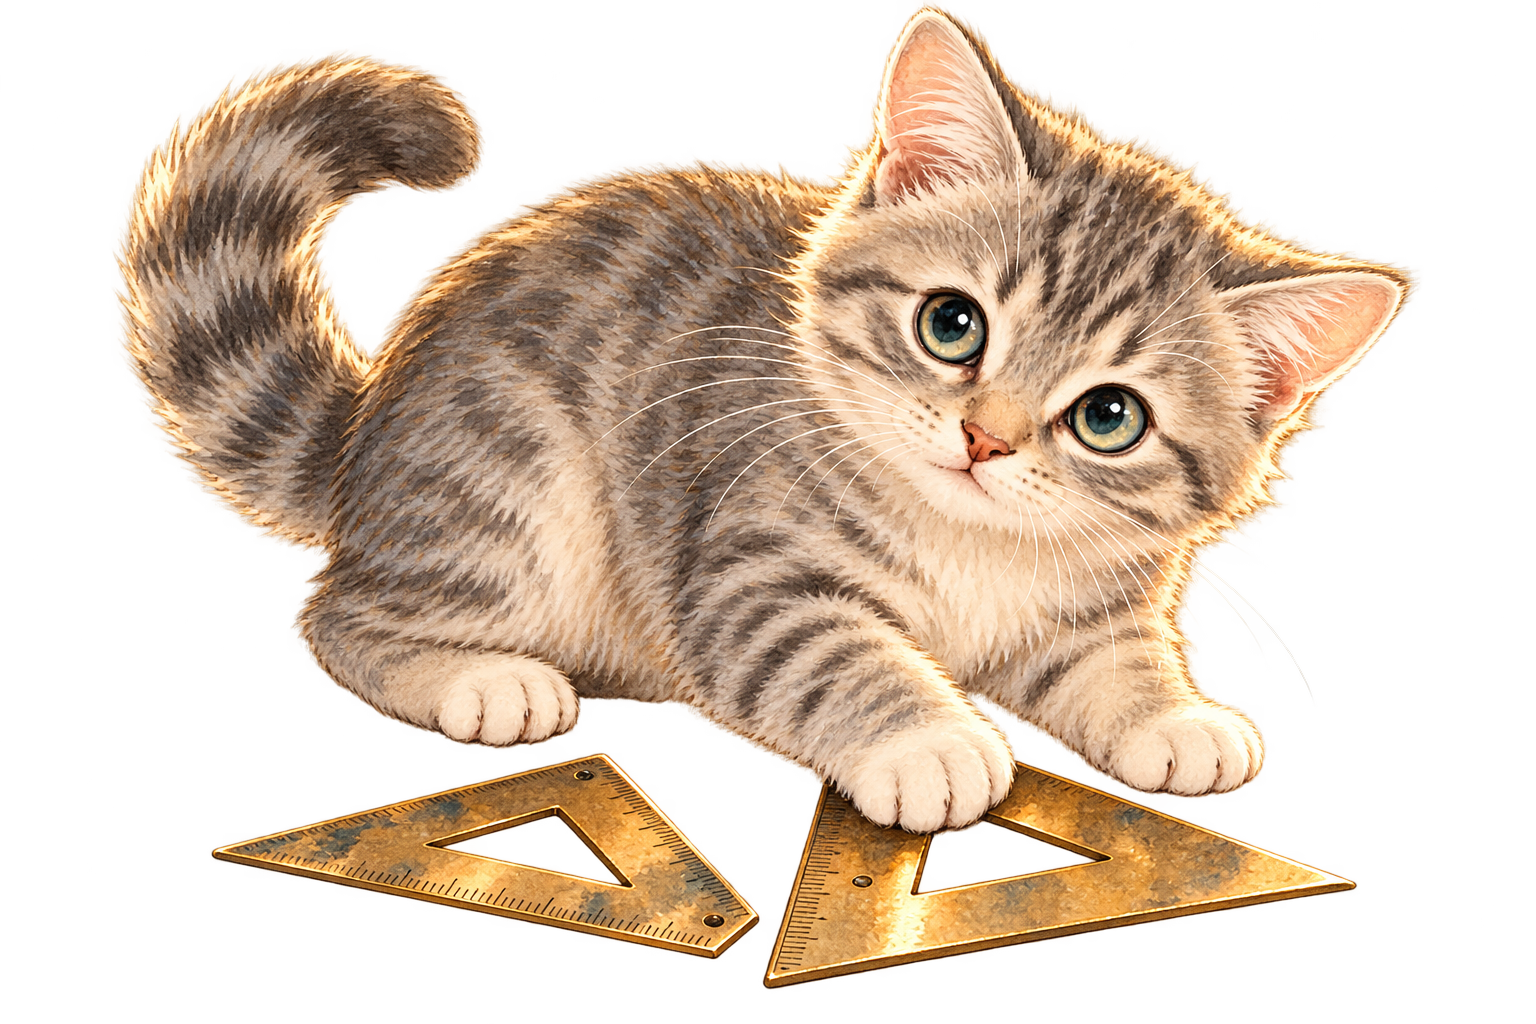
\includegraphics[width=54mm,height=58mm,keepaspectratio]{images/unique/art-68.png}
\end{wrapfigure}
\textit{Доказательство.} Если \(\Delta\ne0\), прямое перемножение в обоих порядках даёт
\[
A\begin{pmatrix}d&-b\\-c&a\end{pmatrix}
=\begin{pmatrix}d&-b\\-c&a\end{pmatrix}A
=\Delta I_2.
\]
Значит, указанная обратная существует. Умножение \(A\mathbf x=\mathbf b\) слева на \(A^{-1}\) даёт единственно возможное \(\mathbf x=A^{-1}\mathbf b\). Оно действительно является решением, так как \(AA^{-1}\mathbf b=\mathbf b\).

Пусть \(\Delta=0\). Если первая строка ненулевая, ненулевой вектор \(\mathbf w=(-b;a)\) удовлетворяет \(A\mathbf w=\mathbf0\). Если первая строка нулевая, но вторая ненулевая, подойдёт \(\mathbf w=(-d;c)\). Для нулевой матрицы можно взять \(\mathbf w=(1;0)\). Обратной быть не может: иначе \(\mathbf w=A^{-1}A\mathbf w=\mathbf0\), что противоречит выбору. Если же некоторое решение \(\mathbf x_0\) системы существует, все различные векторы \(\mathbf x_0+t\mathbf w\), \(t\in\mathbb R\), тоже решения. Поэтому их бесконечно много. Если исходного решения нет, система несовместна.\hfill\(\blacksquare\)
\par\WFclear\end{minipage}\end{lrbox}%
\ifdim\dimexpr\ht\CatFlowBox+\dp\CatFlowBox\relax<64mm\dp\CatFlowBox=\dimexpr64mm-\ht\CatFlowBox\relax\fi%
\noindent\usebox{\CatFlowBox}\par\addvspace{5pt}

Например, \(\begin{pmatrix}1&2\\0&1\end{pmatrix}^{-1}=\begin{pmatrix}1&-2\\0&1\end{pmatrix}\). Два столбца матрицы \(2\times2\) образуют базис плоскости ровно при ненулевом определителе: для любого целевого вектора единственность коэффициентов линейной комбинации — это уже доказанная единственность решения системы. Для больших размеров метод Гаусса остаётся рабочим способом решения, но формулы определителей высших порядков и общая теория базисов требуют отдельного курса.

\par\noindent\begin{minipage}{\linewidth}\section*{Графики}
\begin{center}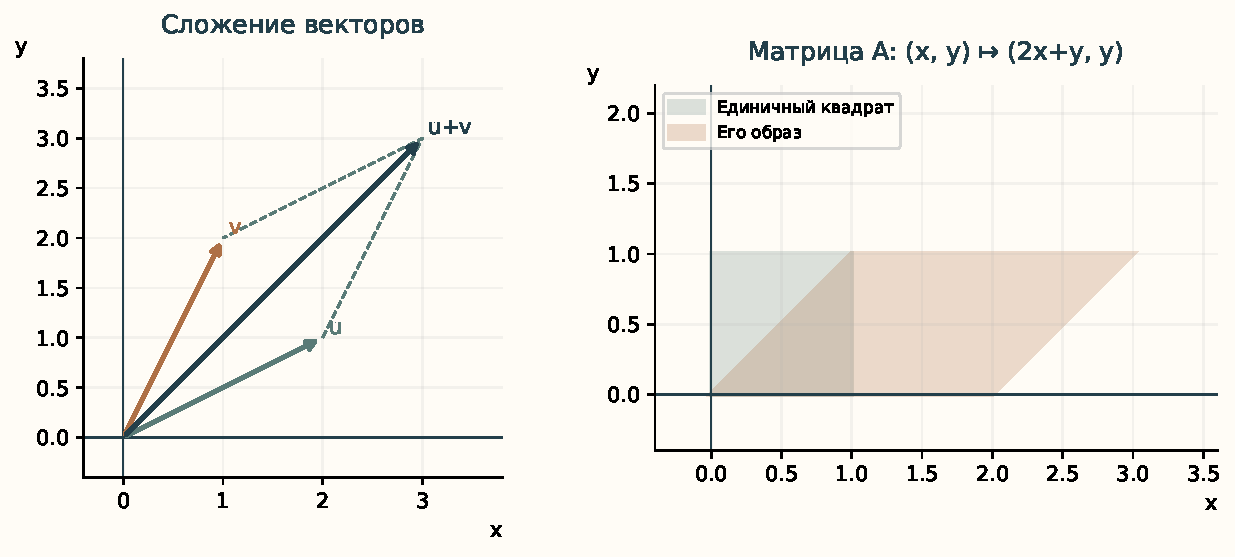
\includegraphics[width=\textwidth,height=.79\textheight,keepaspectratio]{images/atlas-linear.pdf}\par\small Сумма векторов и образ единичного квадрата\end{center}\end{minipage}\par
\Needspace{7\baselineskip}\section*{Задачи}
\begingroup\setlength{\parskip}{3pt}
\noindent\begin{minipage}[t]{\linewidth}\textbf{18.1.} Для \(\mathbf u=(1;-1)\), \(\mathbf v=(3;2)\) найди \(2\mathbf u+\mathbf v\).\par\end{minipage}\par
\noindent\begin{minipage}[t]{\linewidth}\textbf{18.2.} В \(\mathbb R^3\) даны \(\mathbf u=(2;-1;3)\), \(\mathbf v=(-1;4;0)\). Найди \(\mathbf u-\mathbf v\) и \(-2\mathbf v\).\par\end{minipage}\par
\noindent\begin{minipage}[t]{\linewidth}\textbf{18.3.} Точки имеют координаты \(A=(2;-1)\), \(B=(-1;3)\). Найди \(\overrightarrow{AB}\) и расстояние \(AB\).\par\end{minipage}\par
\noindent\begin{minipage}[t]{\linewidth}\textbf{18.4.} Найди длины и скалярное произведение \(\mathbf u=(3;4)\), \(\mathbf v=(4;-3)\). Ортогональны ли векторы?\par\end{minipage}\par
\noindent\begin{minipage}[t]{\linewidth}\textbf{18.5.} Представь \((5;1)\) как \(\alpha(1;1)+\beta(1;-1)\). Найди все возможные коэффициенты.\par\end{minipage}\par
\noindent\begin{minipage}[t]{\linewidth}\textbf{18.6.} Линейно зависимы ли \((2;-3)\) и \((-4;6)\)? Запиши нетривиальную комбинацию, равную нулю.\par\end{minipage}\par
\noindent\begin{minipage}[t]{\linewidth}\textbf{18.7.} Докажи непосредственно по определению, что \((1;2)\) и \((2;1)\) линейно независимы.\par\end{minipage}\par
\noindent\begin{minipage}[t]{\linewidth}\textbf{18.8.} Для \(\mathbf u=(1;0;1)\), \(\mathbf v=(0;1;1)\), \(\mathbf w=(1;1;2)\) найди нетривиальную линейную зависимость.\par\end{minipage}\par
\noindent\begin{minipage}[t]{\linewidth}\textbf{18.9.} Турист прошёл \(3\) км на восток, \(4\) км на север, затем \(1\) км на запад и \(2\) км на юг. Найди вектор итогового перемещения, его длину и общий пройденный путь.\par\end{minipage}\par
\noindent\begin{minipage}[t]{\linewidth}\textbf{18.10.} На тело действуют две силы с координатами \((6;2)\) Н и \((-1;3)\) Н в перпендикулярных осях. Найди равнодействующую и её величину.\par\end{minipage}\par
\noindent\begin{minipage}[t]{\linewidth}\textbf{18.11.} Найди размер матрицы \(A=\begin{pmatrix}1&-1&2\\0&3&1\end{pmatrix}\) и вычисли \(A\begin{pmatrix}2\\1\\-1\end{pmatrix}\).\par\end{minipage}\par
\noindent\begin{minipage}[t]{\linewidth}\textbf{18.12.} Для \(A=\begin{pmatrix}1&1\\0&1\end{pmatrix}\), \(B=\begin{pmatrix}1&0\\1&1\end{pmatrix}\) найди \(AB\) и \(BA\). Равны ли они?\par\end{minipage}\par
\noindent\begin{minipage}[t]{\linewidth}\textbf{18.13.} Для одного набора первого вида нужны \(2\) единицы ингредиента A и \(1\) единица B, для набора второго — \(1\) единица A и \(3\) единицы B. Составь матрицу расхода: строки соответствуют ингредиентам, столбцы — видам наборов. Найди расход для \(4\) наборов первого вида и \(5\) второго.\par\end{minipage}\par
\noindent\begin{minipage}[t]{\linewidth}\textbf{18.14.} Для \(T(x;y)=(2x+y;y)\) найди \(T(1;2)\) и все векторы, переходящие в \((7;3)\).\par\end{minipage}\par
\noindent\begin{minipage}[t]{\linewidth}\textbf{18.15.} Какие отображения \(\mathbb R^2\to\mathbb R^2\) линейны: \(T(x;y)=(2x-y;x+3y)\), \(G(x;y)=(x+1;y)\)? Обоснуй.\par\end{minipage}\par
\noindent\begin{minipage}[t]{\linewidth}\textbf{18.16.} Докажи из определения линейности, что \(T(\mathbf0)=\mathbf0\).\par\end{minipage}\par
\par\addvspace{5pt}\begin{lrbox}{\CatFlowBox}\begin{minipage}[t]{\linewidth}
\setlength{\parskip}{5pt}\setlength{\columnsep}{4.5mm}\setlength{\intextsep}{0pt}
\begin{wrapfigure}[10]{r}{54mm}
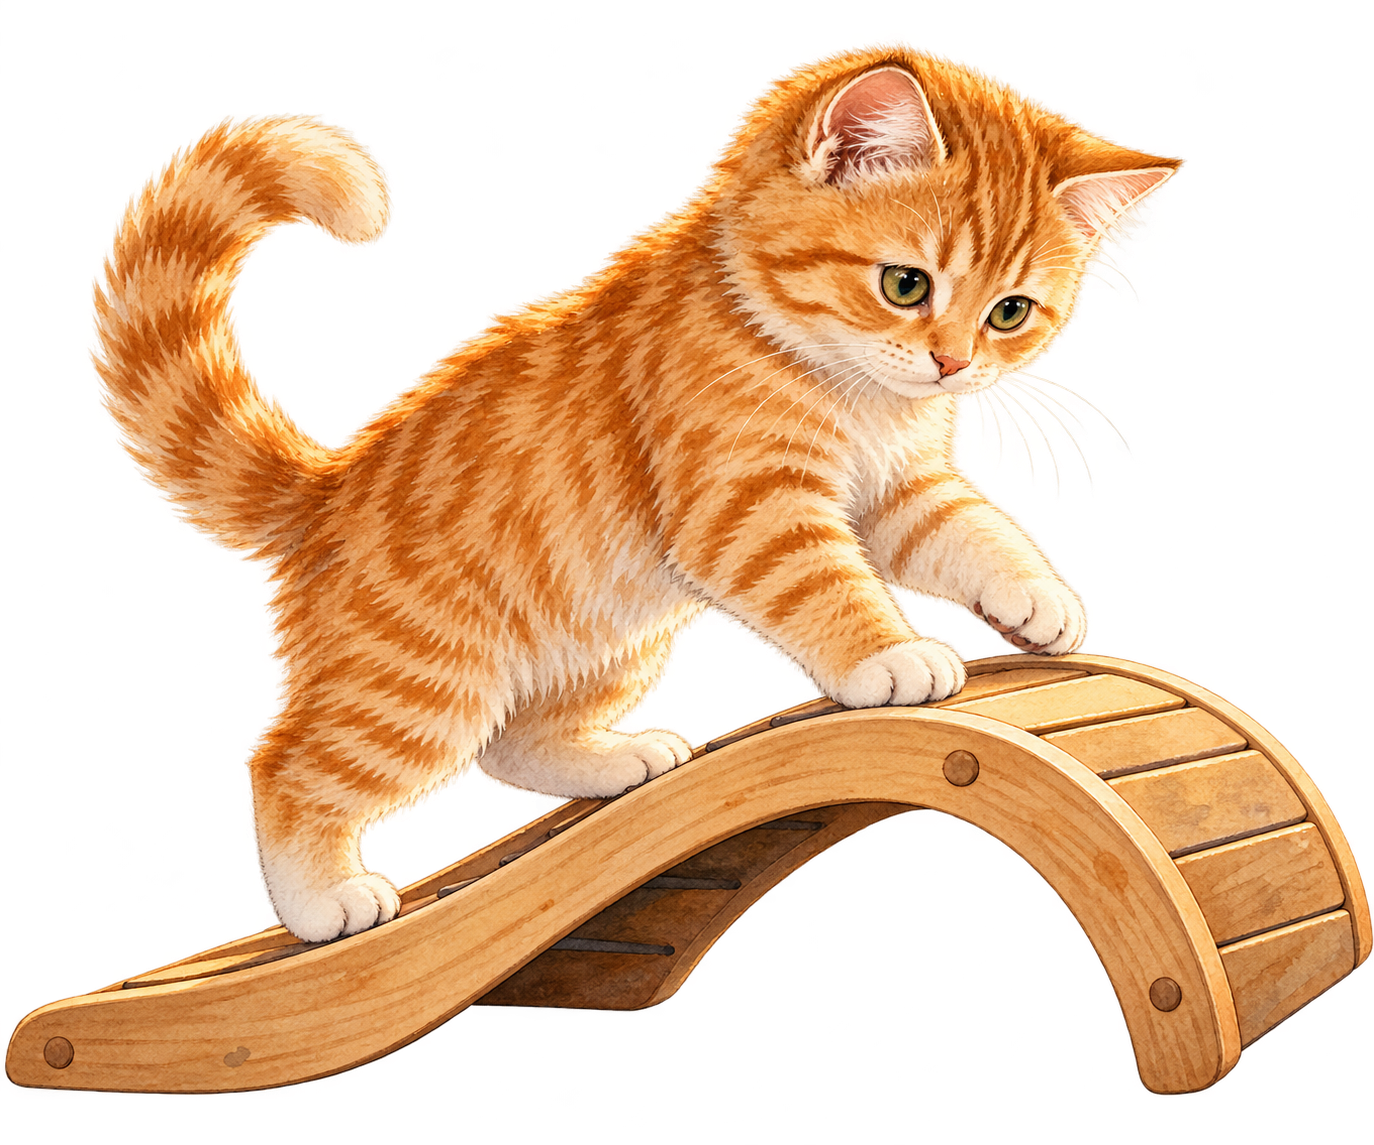
\includegraphics[width=54mm,height=58mm,keepaspectratio]{images/unique/art-49.png}
\end{wrapfigure}
\textbf{18.17.} Для произвольной матрицы \(A=\begin{pmatrix}a&b\\c&d\end{pmatrix}\) докажи вычислением, что \(I_2A=AI_2=A\).\par

\textbf{18.18.} Реши методом исключения \(\begin{cases}2x+y=7,\\x-y=2.\end{cases}\) Укажи преобразование уравнений и проверь ответ.\par

\textbf{18.19.} Опиши все решения системы \(\begin{cases}x+2y=5,\\2x+4y=10.\end{cases}\) Сколько свободных параметров?\par

\textbf{18.20.} Исследуй совместность системы \(\begin{cases}2x-y=4,\\4x-2y=9.\end{cases}\)\par

\textbf{18.21.} Реши методом Гаусса \(\begin{cases}x+y+z=4,\\2x+y+z=6,\\x+2y+3z=9.\end{cases}\)\par

\textbf{18.22.} Опиши все решения \(\begin{cases}x+y+z=4,\\2x+2y+2z=8.\end{cases}\) Сколько свободных параметров?\par

\textbf{18.23.} Для \(A=\begin{pmatrix}3&1\\2&1\end{pmatrix}\) найди определитель и обратную матрицу. С их помощью реши \(A\begin{pmatrix}x\\y\end{pmatrix}=\begin{pmatrix}5\\4\end{pmatrix}\).\par
\par\WFclear\end{minipage}\end{lrbox}%
\ifdim\dimexpr\ht\CatFlowBox+\dp\CatFlowBox\relax<64mm\dp\CatFlowBox=\dimexpr64mm-\ht\CatFlowBox\relax\fi%
\noindent\usebox{\CatFlowBox}\par\addvspace{5pt}

\noindent\begin{minipage}[t]{\linewidth}\textbf{18.24.} Две булочки и один сок стоят \(170\) рублей, одна булочка и два сока — \(160\). Цены одинаковых товаров равны. Составь линейную систему, найди цены и проверь, единственны ли они.\par\end{minipage}\par
\noindent\begin{minipage}[t]{\linewidth}\textbf{18.25.}\starmark{} При всех действительных \(t\) исследуй систему \(\begin{cases}tx+y=1,\\x+ty=1.\end{cases}\) Когда решение единственно, когда решений нет, когда их бесконечно много?\par\end{minipage}\par
\noindent\begin{minipage}[t]{\linewidth}\textbf{18.26.}\starmark{} Приведи к ступенчатому виду систему \(\begin{cases}x+2y-z=1,\\2x+4y-2z=2,\\y+z=2.\end{cases}\) Найди ранг матрицы коэффициентов и все решения.\par\end{minipage}\par
\noindent\begin{minipage}[t]{\linewidth}\textbf{18.27.}\starmark{} Пусть \(A=\begin{pmatrix}1&1\\0&1\end{pmatrix}\). Определим \(A^0=I_2\), а \(A^n\) при натуральном \(n\) — как произведение \(n\) экземпляров \(A\). Докажи индукцией, что \(A^n=\begin{pmatrix}1&n\\0&1\end{pmatrix}\) для всех \(n\in\mathbb N_0\). Найди обратную к \(A^n\).\par\end{minipage}\par
\noindent\begin{minipage}[t]{\linewidth}\textbf{18.28.}\starmark{} Для \(P=\begin{pmatrix}1&0\\0&0\end{pmatrix}\) найди все векторы, удовлетворяющие \(P\mathbf u=\mathbf u\), и все векторы, удовлетворяющие \(P\mathbf u=\mathbf0\). Проверь \(P^2=P\) и объясни, почему обратной матрицы нет.\par\end{minipage}\par
\endgroup
